\documentclass[10pt,a4paper,twoside]{article}
\usepackage[utf8]{inputenc}
\usepackage[english]{babel}
\usepackage{graphicx}
\usepackage{geometry}
\geometry{
 a4paper,
 total={170mm,257mm},
 left=20mm,
 top=20mm,
 }
\usepackage[dvipsnames]{xcolor}
\usepackage{tikz}
\usetikzlibrary{arrows,automata,shapes}
\tikzstyle{decision} = [diamond, draw, fill=blue!20, text width=4.5em, text badly centered, node distance=2.5cm, inner sep=0pt]
\tikzstyle{block} = [rectangle, draw, fill=blue!20, text width=5em, text centered, rounded corners, minimum height=4em]
\tikzstyle{line} = [draw, very thick, color=black!50, -latex']
\tikzstyle{cloud} = [draw, ellipse,fill=red!20, node distance=2.5cm,minimum height=2em]

\author{David Lanzendörfer}
\begin{document}
\section{Well}
\begin{tabular}{c c}
	\hline 
	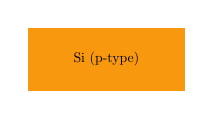
\begin{tikzpicture}[node distance = 3cm, auto, thick,scale=0.5, every node/.style={transform shape}]
		% substrate
		\fill[YellowOrange] (0,0) rectangle (4,1.6);
		\node at (2,0.8) {Si (p-type)};
	\end{tikzpicture} &
	We start with a p-type silicon wafer
	\\ \hline 
	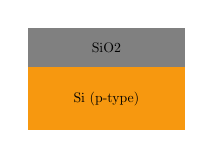
\begin{tikzpicture}[node distance = 3cm, auto, thick,scale=0.5, every node/.style={transform shape}]
		% substrate
		\fill[YellowOrange] (0,0) rectangle (4,1.6);
		\node at (2,0.8) {Si (p-type)};
		% oxide
		\fill[gray] (0,1.6) rectangle (4,2.6);
		\node at (2,2.1) {SiO2};
	\end{tikzpicture} &
	We grow an oxide layer of approximately 1000 angstrom thickness (see documentation)
	\\ \hline 
	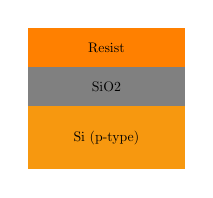
\begin{tikzpicture}[node distance = 3cm, auto, thick,scale=0.5, every node/.style={transform shape}]
		% substrate
		\fill[YellowOrange] (0,0) rectangle (4,1.6);
		\node at (2,0.8) {Si (p-type)};
		% oxide
		\fill[gray] (0,1.6) rectangle (4,2.6);
		\node at (2,2.1) {SiO2};
		% resist
		\fill[orange] (0,2.6) rectangle (4,3.6);
		\node at (2,3.1) {Resist};
	\end{tikzpicture} &
	We thin film deposit a layer of resist
	\\ \hline 
\end{tabular}
\end{document}